\acresetall
\chapter{Evaluation and Results}\label{ch:evaluation}
In this chapter a benchmark of the analyzed algorithms is presented, based on dataset size and complexity. For the first part, the algorithms used for supervised learning are presented, onto which an analysis of the different complexities used is made. From the benchmark, the trained models with the best performance are saved for persistance and then used in the live implementation presented in chapter~\ref{ch:live}.

\section{Performance metrics}\label{ch:performance}

The impact of the dataset size on the algorithm performance is of special interest. Given that the data recorded using the procedure described in section~\ref{ch:measure} has a fixed size, this analysis was performed by slicing the resulting feature extraction files to emulate different dataset sizes. It is important to notice that only slicing for emulate smaller datasets, and not repeating samples for emulation of bigger datasets, has a significant impact in the performance, as noted in section~\ref{ch:size}. This is due to the fact that repeated samples present no new information to the model, and there is nothing new to learn from them.

The dataset is, then, sliced into four different sizes:

\begin{itemize}
    \item Small dataset (S): is one fourth (1/4) of the original dataset
    \item Medium dataset (M): is one third (1/3) of the original dataset
    \item Large dataset (L): is half (1/2) of the original dataset
    \item Extra Large dataset (XL): the whole set of features extracted as recorded from the signals over the air.
\end{itemize}

Furthermore, a benchmark of the learning algorithms is made based on variations on their complexities. Each algorithm has different ways to represent its own complexity, and this has a significant impact over its overall performance. The \ac{ML} algorithms used in this analysis are: K-nearest neighbors, \ac{SVM} and binary tree classificators. Their complexities are set as follows:

\begin{itemize}
    \item K-nearest neighbors: the complexity of this algorithm is set by the amount of neighbors that are considered in order to make a classification decision. For the benchmark, different models were trained using 2, 4, 10 and 50 neighbors.
    \item \ac{SVM}: this algorithm allows the designer to select the type of kernel that is used during the learning process. The function of the kernel is to generate internally non-linear transformations over the input data while still behaving as a linear classificator. For this work, the \ac{RBF} is used as a kernel because of its known good performance on multiclass classification problems at the cost of longer training times. The complexity of this model is then set by providing different values to the 'C' parameter of this \ac{RBF} kernel. This parameter sets the trade off between the proneness of the model to result in a erroneous classification and the simplicity of the decision boundary. For this work, values of C=(1, 1000, 1000000) are given.
    \item Decision Trees: in this model, the complexity is ruled by the depth of the decision branch. Here, depths of 2, 5, 10 and 50 are given.
\end{itemize}

Moreover, it is also interesting to determine how the models behave when the features have been scaled. A first glance of the impact of a scaler is presented by using the StandardScaler() from SKlearn, which simply removes the mean of the features and scales them to unit variance. A side-by-side comparison on model performance when trained with unscaled features vs.scaled features is shown as a result from the benchmark. The results are depicted in Figs~\ref{fig:knn}, \ref{fig:dtc} and \ref{fig:svc}.

\begin{figure}[!htb]
    \centering
    \begin{subfigure}[htb]{0.49\textwidth}
        \centering
        \includestandalone[width=\linewidth]{figures/knn_accs}
        \label{fig:knn_accs}
    \end{subfigure}
    \begin{subfigure}[htb]{0.49\textwidth}
        \centering
        \includestandalone[width=\linewidth]{figures/knn_accs_scaled}
        \caption{Accuracy with scaled features}
        \label{fig:knn_accs_scaled}
    \end{subfigure}\\
    \begin{subfigure}[htb]{0.49\textwidth}
        \centering
        \includestandalone[width=\linewidth]{figures/knn_fit_times}
        \caption{Training times with unscaled features}
        \label{fig:knn_fit_times}
    \end{subfigure}
    \begin{subfigure}[htb]{0.49\textwidth}
        \centering
        \includestandalone[width=\linewidth]{figures/knn_fit_times_scaled}
        \caption{Training times with scaled features}
        \label{fig:knn_fit_times_scaled}
    \end{subfigure}\\
    \begin{subfigure}[htb]{0.49\textwidth}
        \centering
        \includestandalone[width=\linewidth]{figures/knn_pred_times}
        \caption{Prediction times with unscaled features}
        \label{fig:knn_pred_times}
    \end{subfigure}
    \begin{subfigure}[htb]{0.49\textwidth}
        \centering
        \includestandalone[width=\linewidth]{figures/knn_pred_times_scaled}
        \caption{Prediction times with scaled features}
        \label{fig:knn_pred_times_scaled}
    \end{subfigure}
    \caption{K-nearest Neighbors}
    \label{fig:knn}
\end{figure}

\begin{figure}[!htb]
    \centering
    \begin{subfigure}[htb]{0.49\textwidth}
        \centering
        \includestandalone[width=\linewidth]{figures/dtc_accs}
        \caption{Accuracy with unscaled features}
        \label{fig:dtc_accs}
    \end{subfigure}
    \begin{subfigure}[htb]{0.49\textwidth}
        \centering
        \includestandalone[width=\linewidth]{figures/dtc_accs_scaled}
        \caption{Accuracy with scaled features}
        \label{fig:dtc_accs_scaled}
    \end{subfigure}
    \begin{subfigure}[htb]{0.49\textwidth}
        \centering
        \includestandalone[width=\linewidth]{figures/dtc_fit_times}
        \caption{Training times with unscaled features}
        \label{fig:dtc_fit_times}
    \end{subfigure}
    \begin{subfigure}[htb]{0.49\textwidth}
        \centering
        \includestandalone[width=\linewidth]{figures/dtc_fit_times_scaled}
        \caption{Training times with scaled features}
        \label{fig:dtc_fit_times_scaled}
    \end{subfigure}
    \begin{subfigure}[htb]{0.49\textwidth}
        \centering
        \includestandalone[width=\linewidth]{figures/dtc_pred_times}
        \caption{Prediction times with unscaled features}
        \label{fig:dtc_pred_times}
    \end{subfigure}
    \begin{subfigure}[htb]{0.49\textwidth}
        \centering
        \includestandalone[width=\linewidth]{figures/dtc_pred_times_scaled}
        \caption{Prediction times with scaled features}
        \label{fig:dtc_pred_times_scaled}
    \end{subfigure}
    \caption{Decision Trees}
    \label{fig:dtc}
\end{figure}

\begin{figure}
    \centering
    \begin{subfigure}[htb]{0.49\textwidth}
        \centering
        \includestandalone[width=\linewidth]{figures/svc_accs}
        \caption{Accuracy with unscaled features}
        \label{fig:svc_accs}
    \end{subfigure}
    \begin{subfigure}[htb]{0.49\textwidth}
        \centering
        \includestandalone[width=\linewidth]{figures/svc_accs_scaled}
        \caption{Accuracy with scaled features}
        \label{fig:svc_accs_scaled}
    \end{subfigure}
    \begin{subfigure}[b]{0.49\textwidth}
        \centering
        \includestandalone[width=\linewidth]{figures/svc_fit_times}
        \caption{Training times with unscaled features}
        \label{fig:svc_fit_times}
    \end{subfigure}
    \begin{subfigure}[b]{0.49\textwidth}
        \centering
        \includestandalone[width=\linewidth]{figures/svc_fit_times_scaled}
        \caption{Training times with scaled features}
        \label{fig:svc_fit_times_scaled}
    \end{subfigure}
    \begin{subfigure}[b]{0.49\textwidth}
        \centering
        \includestandalone[width=\linewidth]{figures/svc_pred_times}
        \caption{Prediction times with unscaled features}
        \label{fig:svc_pred_times}
    \end{subfigure}
    \begin{subfigure}[b]{0.49\textwidth}
        \centering
        \includestandalone[width=\linewidth]{figures/svc_pred_times_scaled}
        \caption{Prediction times with scaled features}
        \label{fig:dtc_pred_times_scaled}
    \end{subfigure}
    \caption{Support Vector Machines}
    \label{fig:svc}
\end{figure}

From Figs~\ref{fig:knn}, \ref{fig:dtc} and \ref{fig:svc} a couple of conclusions can be extracted. First, it is seen that the accuracy of the model increases as more data is taken into consideration, which is well according with the theory and serves as queue for applying the same implementation with more data as proposed in chapter~\ref{ch:conclusions}. Furthermore, three different behaviours are appreciated:

\begin{itemize}
    \item: As complexity increases, the K-nearest neighbors algorithm shows a decrease on its overall accuracy, which is an indication that the model is overfitting, and suggests that with such a complexity (50 neighbors, in this case), the model is starting to "memorize" characteristics of the training dataset, and is set to perform badly if unknown samples are feed to it, as its capabilities for generalization are in decay. Moreover, the prediction times for the highest level of complexity are already about two times greater than the second highest, making it not suitable for live implementations. Furthermore, this model shows a both a reduction in accuracy as well as an increase in prediction time when the features have been scaled, which simply states that the model performs well without further data preprocessing right after the feature extraction.
    \item The decision tree model shows a steady increase on its accuracy as complexity increases, without reaching a clear overfitting state. Complexity has a clear effect on the training times, but it is still on the range of the milliseconds - being a process done only once, this does not affect dramatically the model selection and does not closes the possibility of increasing the complexity for this specific use case. This can also be backed on the fact that  the prediction times seem to stay constant with this increase. Interestingly, not only the training times are reduced after scaling, but also the prediction times are drastically improved, reaching about 10x faster predictions using the standard scaler. With comparable accuracy, scaling the features seems like a prospect procedure when this model is used in time demanding or live implementations.
    \item the \ac{SVM} do not show a clear tendency to improve as complexity is increased, and just like the K-nearest neighbor models, performs quite well in small sizes of datasets. However, the best accuracy for this model is still below the accuracies of the other models regarded in this benchmark. Additionally, the training and prediction times exceed dramatically the times achieved with the other models, being about 8000 longer for training and around 500 times longer for prediction. The fact that this model is that slow will definitely affect considerably the performance of realtime implementations, aspect that is crucial in systems such as cognitive radio.
\end{itemize}

\section{Scenario Classification}
Besides of the general performance that the learning models have in regard of the whole testing set, it is paramount to determine how good they perform by classifing each of the specific scenarios of Table~\ref{table:scenarios}. To assess this, confusion matrices are used to determine the amount of rightfully classified scenarios, along with the false possitives and false negatives. On this analysis, it is only of interest the amount of correctly classified scenarios, and any misclassification affects the implementation equally, regardless of its type. Moreover, in section~\ref{ch:performance} can be seen that each algorithm behaves differently in terms not only of accuracy, but also in training time and prediction time. As the models are trained only once, the "training time" does not play a role in the model selection for this work, as it does not have any repercussion on the performance of the model when new values are applied to it. Therefore, "prediction time" and "accuracy" are metrics of quality that are considered for this models on its selection to be applied on real time scenarios.\\

Confusion matrices show how each of the samples from the data set are classified for a given model. As a matter of ilustration, a side by side comparison for the worst-performing vs. the best-performing model, with respect to accuracy, is given in Fig~\ref{fig:confusionknn}, \ref{fig:confusiondtc} and \ref{fig:confusionsvc}. The complete set of confusion matrices, corresponding to every trained model, can be found at the development notebook for this work \cite{repo:cognitive_radio_ml}.


\begin{figure}[!htb]
    \captionsetup[subfigure]{justification=centering}
    \centering
    \begin{subfigure}[htb]{0.49\textwidth}
        \centering
        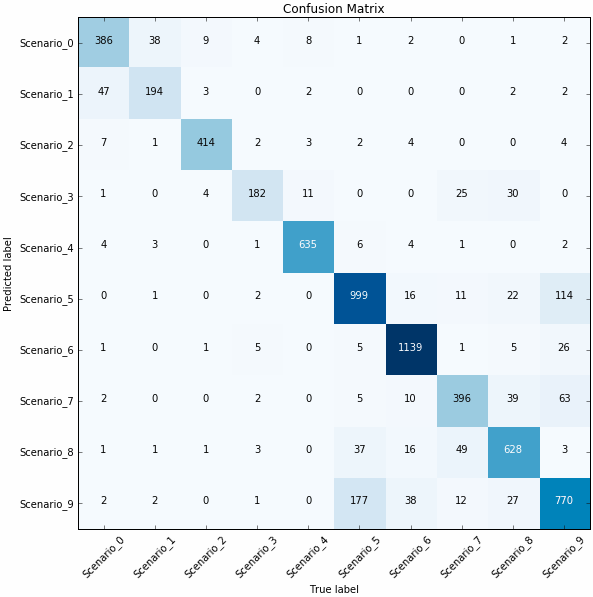
\includegraphics[width=\linewidth]{figures/knn_scaled_S_50}
        \caption{KNN-50 neighbors, StandardScaled, trained with small (S) dataset}
        \label{fig:knn_2}
    \end{subfigure}
    \begin{subfigure}[htb]{0.49\textwidth}
        \centering
        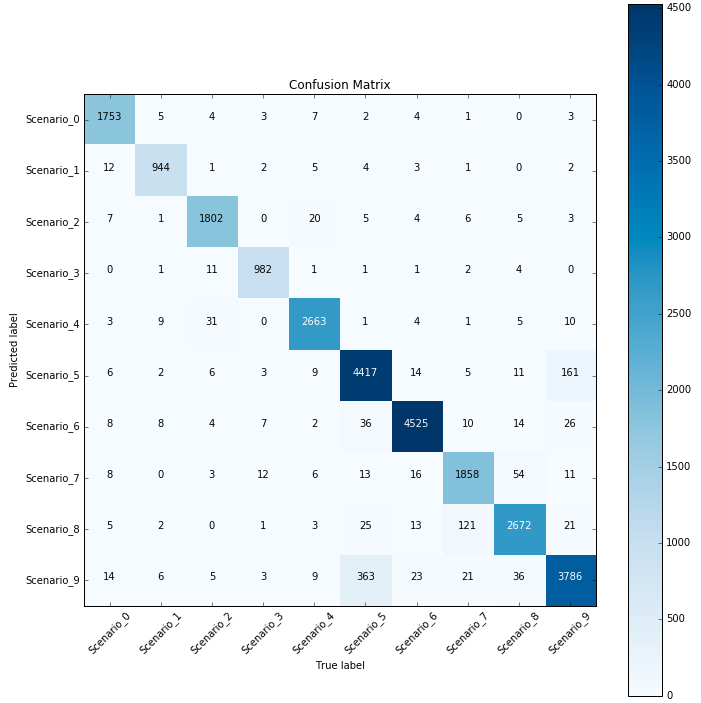
\includegraphics[width=\linewidth]{figures/knn_unscaled_XL_4}
        \caption{KNN-4 neighbors, unscaled, trained with whole (XL) dataset}
        \label{fig:knn_4}
    \end{subfigure}
    \caption{Confusion Matrixes for K-nearest Neighbor Models}
    \label{fig:confusionknn}
\end{figure}

\begin{figure}[!htb]
    \captionsetup[subfigure]{justification=centering}
    \centering
    \begin{subfigure}[htb]{0.49\textwidth}
        \centering
        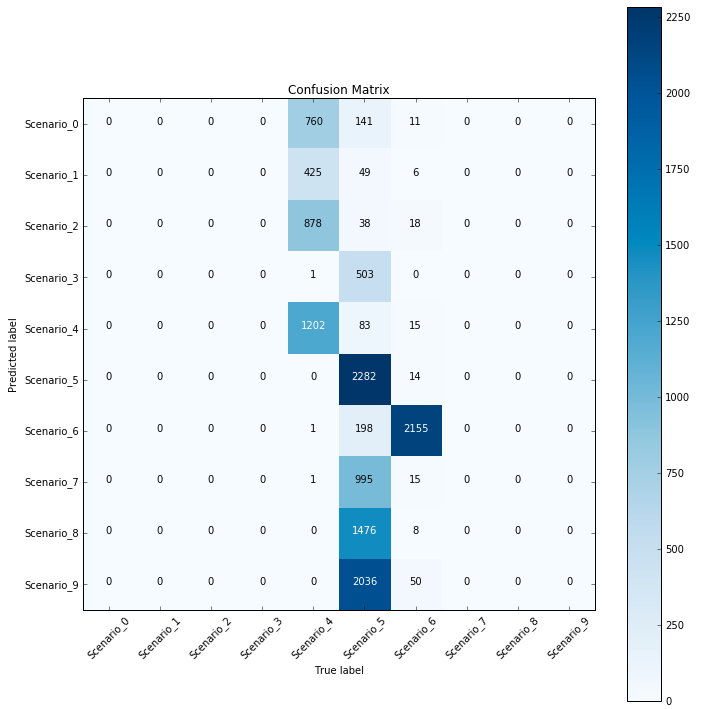
\includegraphics[width=\linewidth]{figures/dtc_unscaled_L_2}
        \caption{Decision Tree, unscaled, depth=2, trained with large (L) dataset}
        \label{fig:knn_2}
    \end{subfigure}
    \begin{subfigure}[htb]{0.49\textwidth}
        \centering
        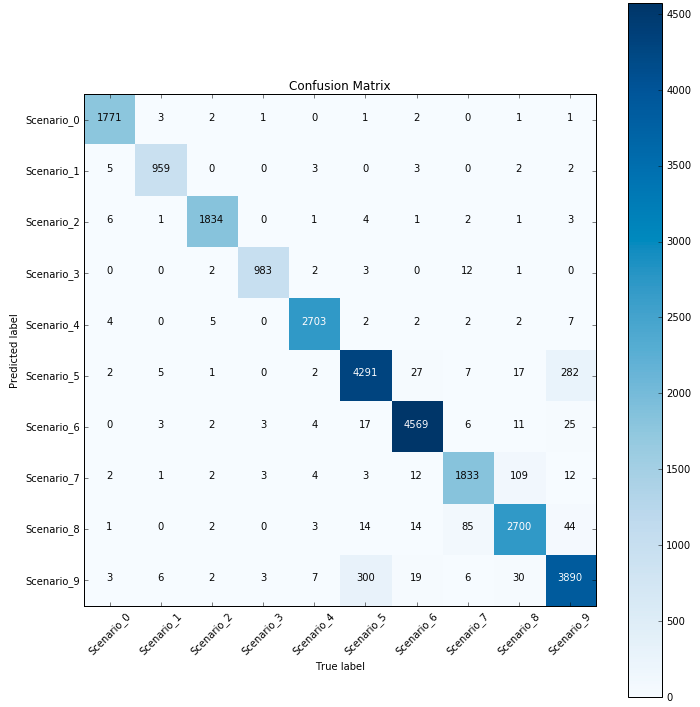
\includegraphics[width=\linewidth]{figures/dtc_unscaled_XL_50}
        \caption{Decision Tree, unscaled, depth=50, trained with whole (XL) dataset}
        \label{fig:knn_4}
    \end{subfigure}
    \caption{Confusion Matrixes for Decision Tree Models}
    \label{fig:confusiondtc}
\end{figure}
\begin{figure}[!htb]
    \captionsetup[subfigure]{justification=centering}
    \centering
    \begin{subfigure}[htb]{0.49\textwidth}
        \centering
        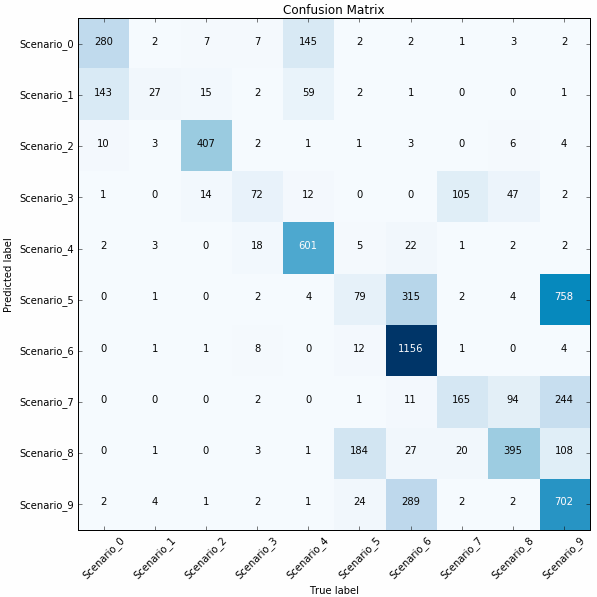
\includegraphics[width=\linewidth]{figures/svc_scaled_S_1}
        \caption{\ac{SVM}, StandardScaled, C=1, trained with small (S) dataset}
        \label{fig:knn_2}
    \end{subfigure}
    \begin{subfigure}[htb]{0.49\textwidth}
        \centering
        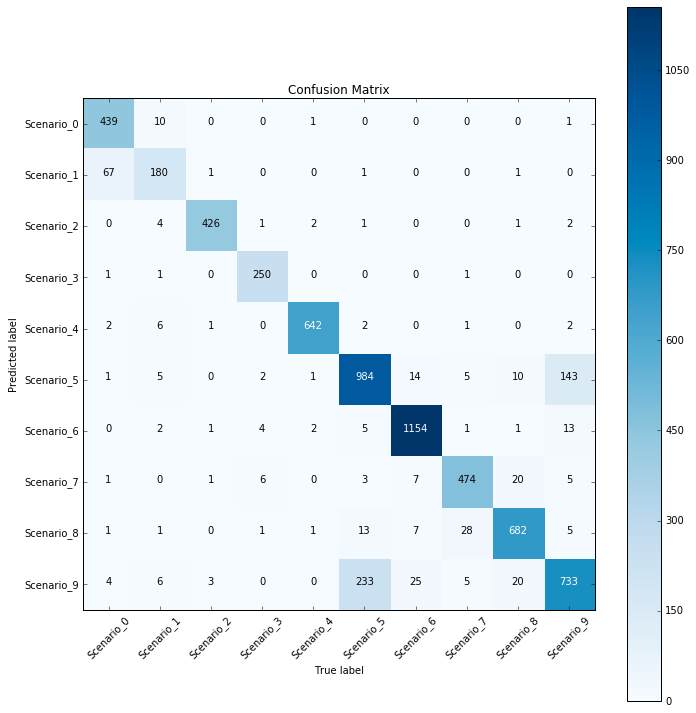
\includegraphics[width=\linewidth]{figures/svc_scaled_S_1e6}
        \caption{\ac{SVM}, StandardScaled, C=1e6, trained with small (S) dataset}
        \label{fig:knn_4}
    \end{subfigure}
    \caption{Confusion Matrixes for \ac{SVM} Models}
    \label{fig:confusionsvc}
\end{figure}
It is also important to notice the clear difference on the number of samples present for each scenario. This is due to the fact that the measurements performed in section~\ref{ch:measure} were based on runtime and not on number of generated samples, and the feature extraction algorithm described in section~\ref{ch:features} generates a different number of samples for each scenario, because of its dependence on the \emph{frame events} generation consequent of the channel ocuppation and interframe time of arrival itself. A different approach for feature extraction based on number of features generated is proposed in chapter~\ref{ch:conclusions}.

From these matrices it can be clearly seen, on a first glance, that the K-nearest algorithm performs quite well regardless of its configuration, having a more populated diagonal in its confusion matrix in comparison with the other two analyzed models. Additionally, just a small improvement in the classification accuracy is seen as the complexity and dataset size increases for this model. In general, it is safe to assert that the classification performs generally well for most of the scenarios except from scenario 5, where a higher number of false positives as well as false negatives is seen for all models, being missclassified as scenario 9. This indicates that the extracted features for these specific scenarios have a noticeable correlation, and serve as an invitation to determine a feature that confidently sets a difference between them.

Based on this analysis, one model of each kind is selected to be implemented on realtime samples. The selected models are those who have the best trade-off between accuracy and prediction time. The selected models are:

\begin{itemize}
    \item K-nearest neighbors with 4 neighbors, trained with XL unscaled dataset.
    \item Decision tree with a tree depth=50, trained with XL scaled dataset using a standard scaler.
    \item \ac{SVM} with an RBF complexity of 1e6, trained with S  scaled dataset using a standard scaler.
\end{itemize}


\begin{figure}[!htb]
    \centering
    \begin{subfigure}[htb]{0.49\textwidth}
        \centering
        \begin{tikzpicture}[scale=0.9]
            \begin{axis}[
                xlabel={Iterations},
                ylabel={Loss Factor \%},
                  ]
                \addplot table [x=epoch, y=loss, col sep=comma, mark=none] {data/adadelta.csv};
                \addplot table [x=epoch, y=val_loss, col sep=comma, mark=none] {data/adadelta.csv};
                \legend{Training loss, Validation loss}
        \end{axis}
        \end{tikzpicture}
    \end{subfigure}
    \hfill
    \begin{subfigure}[htb]{0.49\textwidth}
        \centering
        \begin{tikzpicture}[scale=0.9]
            \begin{axis}[legend pos=south east,
                xlabel={Iterations},
                ylabel={Accuracy \%},
                  ]
                \addplot table [x=epoch, y=acc, col sep=comma, mark=none] {data/adadelta.csv};
                \addplot table [x=epoch, y=val_acc, col sep=comma, mark=none] {data/adadelta.csv};
                \legend{Accuracy, Validation Accuracy}
        \end{axis}
        \end{tikzpicture}
    %}
    \end{subfigure}
    \caption{Metrics for Adadelta Optimizer}
    \label{fig:adadelta}
\end{figure}

\begin{figure}[!htb]
    \centering
    \begin{subfigure}[htb]{0.49\textwidth}
        \centering
        \begin{tikzpicture}[scale=0.8]
            \begin{axis}[
                xlabel={Iterations},
                ylabel={Loss Factor \%},
                  ]
                \addplot table [x=epoch, y=loss, col sep=comma, mark=none] {data/adamax.csv};
                \addplot table [x=epoch, y=val_loss, col sep=comma, mark=none] {data/adamax.csv};
                \legend{Training loss, Validation loss}
        \end{axis}
        \end{tikzpicture}
    \end{subfigure}
        \hfill
    \begin{subfigure}[htb]{0.49\textwidth}
        \centering
        \begin{tikzpicture}[scale=0.8]
            \begin{axis}[legend pos=south east,
                xlabel={Iterations},
                ylabel={Accuracy \%},
                  ]
                \addplot table [x=epoch, y=acc, col sep=comma, mark=none] {data/adamax.csv};
                \addplot table [x=epoch, y=val_acc, col sep=comma, mark=none] {data/adamax.csv};
                \legend{Accuracy, Validation Accuracy}
        \end{axis}
        \end{tikzpicture}
    \end{subfigure}
    \caption{Metrics for Adamax Optimizer}
    \label{fig:adamax}
\end{figure}

\begin{figure}[!htb]
    \centering
    \begin{subfigure}[htb]{0.49\textwidth}
        \centering
        \begin{tikzpicture}[scale=0.8]
            \begin{axis}[
                xlabel={Iterations},
                ylabel={Loss Factor \%},
                  ]
                \addplot table [x=epoch, y=loss, col sep=comma, mark=none] {data/sgd.csv};
                \addplot table [x=epoch, y=val_loss, col sep=comma, mark=none] {data/sgd.csv};
                \legend{Training loss, Validation loss}
        \end{axis}
        \end{tikzpicture}
    \end{subfigure}
        \hfill
    \begin{subfigure}[htb]{0.49\textwidth}
        \centering
        \begin{tikzpicture}[scale=0.8]
            \begin{axis}[legend pos=south east,
                xlabel={Iterations},
                ylabel={Accuracy \%},
                  ]
                \addplot table [x=epoch, y=acc, col sep=comma, mark=none] {data/sgd.csv};
                \addplot table [x=epoch, y=val_acc, col sep=comma, mark=none] {data/sgd.csv};
                \legend{Accuracy, Validation Accuracy}
        \end{axis}
        \end{tikzpicture}
    \end{subfigure}
    \caption{Metrics for Steepest Gradient descent Optimizer}
    \label{fig:adadelta}
\end{figure}
\section{Dyspan setup comparison}
